\documentclass[a4paper]{article}
\usepackage[a4paper, margin=2.5cm]{geometry}
\usepackage[utf8]{inputenc}
\usepackage[T1]{fontenc}
\usepackage{graphicx}
\usepackage[english]{babel}
\usepackage{hyperref}
\usepackage{float}
\usepackage{amsthm}
\usepackage{amsmath}
\usepackage{multicol}
\usepackage{wrapfig}
\usepackage{bm}
\usepackage{amssymb}
\usepackage{listings}
\usepackage{minted}
\usepackage{tikz}
\usetikzlibrary{calc,arrows.meta,positioning, automata, shapes}
\usepackage[]{algorithm2e}
\usepackage{paralist}

\hypersetup{
    colorlinks = true,
    citecolor = black,
    urlcolor = blue,
    linkcolor = black,
}
\usepackage[
    backend=biber,
    style=alphabetic,
    citestyle=authoryear
]{biblatex}
\usepackage{csquotes}
\addbibresource{ref.bib}

\newcommand{\question}[2]{
\paragraph{Question #1} -- \textit{#2}

}
\newcommand{\programming}[1]{
\paragraph{Programming} -- \textit{#1}

}

\title{Reinforcement Learning Lab Session 8}
\author{Dawid Miroyan}

\begin{document}
\maketitle
\section*{Introduction}
In this document we will study the "Actor-Critic" Reinforcement Learning method on different environments. These methods are \textbf{A2C} and \textbf{PPO} on the Cartpole-v1 and LunarLander-v2 environments.

In these "Actor-Critic" methods two nueral networks will be used:
\begin{itemize}
\item \textbf{Actor:} Controls how our agent behaves (policy-based)
\item \textbf{Critic:} Measures how good the state is (vlaue-based)
\end{itemize}

The Critic observes the taken actions and provides feedback. The Actor uses this feedback to update it's policy.
Meanwhile the Critic will update their own way to provide feedback so it can be better next time.

\tableofcontents
\newpage

\section{Difference between A2C and PPO}
The main difference between A2C and PPO (Proximal Policy Optimiziation) is that for PPO we will avoid having too large policy updates. This improves the stability of the Actor training.


\section{Solving the LunarLander-v2 environment}

\begin{figure}[H]
    \centering
    % Change the plot name here:
    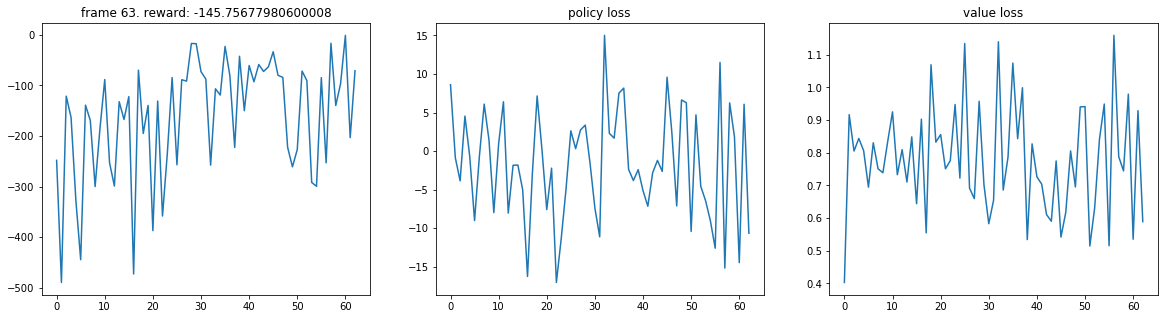
\includegraphics[width=\linewidth]{plots/LL_A2C.png}
    \caption{Reward, policy and value loss when training on the LunarLander environment using A2C.}
    \label{fig:LL_A2C}
\end{figure}

\begin{figure}[H]
    \centering
    % Change the plot name here:
    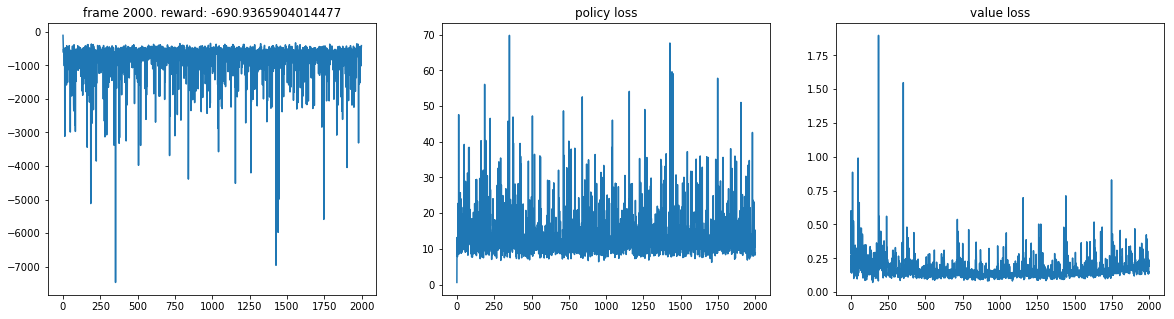
\includegraphics[width=\linewidth]{plots/LL_PPO.png}
    \caption{Reward, policy and value loss when training on the LunarLander environment using PPO.}
    \label{fig:LL_PPO}
\end{figure}


\section{Performance comparison}

\section{Potential improvements}


\printbibliography
\end{document}

